\chapter{OTHER PHYSICAL PROCESSES}
% !TEX root = hazy3.tex

\section{Overview}

This section describes other physics processes that have been incorporated
into \Cloudy.  Some of these are taken from published papers that have
described the formalism used by \Cloudy\ in detail.
The original papers are
cited in the beginning of each section.

\section{Magnetic fields}

Magnetic fields are not normally considered by the code, but can be
included with the \cdCommand{magnetic field} command.

Cooling due to electron cyclotron emission, using equations from
\citet{Fabian1976}; these assume optically thin emission) are included
when the field is specified.  The volume-cooling rate is given by
\begin{equation}
\Lambda_{cyclotron} = n_e \frac{B^2}{8\pi} \frac{4}{3}
\sigma_{Thom}c\left(\frac{v_e}{c}\right)^2= 4.5433\times 10^{-25} n_e B^2T_e
\quad [\mathrm{erg~cm}^{-3} \mathrm{s}^{-1}]
\end{equation}
where $\sigma_T$ is the Thomson cross-section and
\begin{equation}
{u_e} = {\left( {\frac{{8k{T_e}}}{{\pi \,{m_e}}}} \right)^{1/2}} = 6.2124
\times {10^5}\,T_e^{1/2}\quad
 [\mathrm{cm~s}^{-1}]
\end{equation}
is the mean electron speed.
See, however, \citet{Masters1977}.
They show that this emission process is likely to be optically
thick under some circumstances.  Cyclotron optical depth effects are not
now treated, so this cooling rate is likely to be an overestimate.

Magnetic pressure is included in the gas equation of state.\footnote{The pressure associated with the magnetic field was not included
in the total pressure in versions 95 and earlier of the code.}
The magnetic pressure  in the general case will be
\begin{equation}
{P_{mag}} = \frac{{B_{{\mathrm{tangled}}}^{\mathrm{2}}}}{{8\pi }} +
\frac{{B_{{\mathrm{tangential}}}^{\mathrm{2}} - B_{{\mathrm{parallel}}}^{\mathrm{2}}}}{{8\pi
}}\quad  [\mathrm{dynes~cm}^{-2}]\   [\mathrm{erg~cm}^{-3}].
\end{equation}
and the enthalpy density is
\begin{equation}
\label{eqn:MagneticFieldEnthalpyDensity}
{w_{mag}} = \frac{\gamma }{{\gamma  -
1}}\frac{{B_{{\mathrm{tangled}}}^{\mathrm{2}}}}{{8\pi }} +
\frac{{B_{{\mathrm{tangential}}}^{\mathrm{2}} + B_{{\mathrm{parallel}}}^{\mathrm{2}}}}{{4\pi
}}
\quad [\mathrm{dynes~cm}^{-2}]\  [\mathrm{erg~cm}^{-3}].
\end{equation}

The field strength is determined from local conditions across the cloud.
A tangled field will have a strength that is related to the local density
by equation \ref{eqn:MagneticFieldEnthalpyDensity}.
To force a constant magnetic field specify $\gamma = 0$.
An ordered
field is assumed to have constant strength if the gas is stationary.
If
the gas is moving (a wind solution is being performed) then the component
in the radial direction (the parallel component) is constant and the
transverse field has a strength that is given by (\citealp{Cowling1976})
\begin{equation}
{B_t} = B_t^0\frac{{u_o^2 - u_A^2}}{{u{u_0} - u_A^2}}.
\end{equation}
where $u_A^{}$
 is the Alfv\'en velocity at illuminated face,
\begin{equation}
u_A^2 = \frac{{B_{parallel}^2}}{{4\pi {\rho _0}}}
\quad  [\mathrm{cm}^2 \mathrm{s}^{-2}].
\end{equation}

For reference, a tangled field will have a pressure equivalent to the
thermal pressure of a gas with density $n$ and temperature $T$ when
\begin{equation}
P_{mag}/k=\frac{B^2}{8\pi} \frac{1}{k} = B^2 2.882\times 10^{14}\approx nT
\quad  [\mathrm{cm}^{-3} \mathrm{K}].
\end{equation}
In the ISM this magnetic pressure is often roughly equal to the ram or
turbulent pressure
\begin{equation}
P_{ra,}/k=pu^2 / 2k=60.14 nu_{km~s^{-1}}^2 \approx nT
\quad [\mathrm{cm}^{-3} \mathrm{K}].
\end{equation}
where the last velocity is in km/s and $n$ is the nucleon density (cm$^{-3}$).
For comparison, the Alfv\'en velocity, the speed at which magnetic fields
convey information, is
\begin{equation}
u_A = \frac{B}{(4\pi \rho)^{1/2}} \approx 2.19 \times 10^6B n^{-1/2}
\quad [\mathrm{km~s}^{-1}].
\end{equation}

Cosmic rays should not be included when a magnetic field is specified,
since the effects of a field on cosmic ray transport are not now treated.
A warning will be printed if both are included.

\section{Cosmic ray interactions}

The implementation of cosmic rays was done in collaboration with Richard
Mushotzky.
This section is taken from \citet{FerlandMushotzky1984}.

Synchrotron radio sources are usually modeled in terms of an interaction
between a magnetic field and a relativistic gas with a typical energy per
electron of a few hundred MeV (see \citealp{Pacholczyk1970}; \citealp{Longair1981}).
The
spectral index of the radio emission for radio-loud active galaxies is
usually $\sim -0.7$, and this suggests that the electrons, which make the dominant
contribution to synchrotron emission, have a density (per unit energy
interval) given by $n(cr, E)\sim  E^{-2.4}$ (\citealp{Kellerman1966}).  The total relativistic
electron density is sensitive to the lower bound of the energy distribution,
which is typically of order 10--100 MeV,
corresponding to relativistic factor
of  $\gamma\sim 10-100$ \citep{Lea1978}.

The cosmic ray density used by \Cloudy\ is defined as
\begin{equation}
n(cr) = \int_{{E_{\min }}}^{{E_{\max }}} {n\left( {cr,\;E} \right)\;dE}
\quad  [\mathrm{cm}^{-3}]
\end{equation}
with the lower bound set to $E_{\mathrm{min}} = 5$ MeV, corresponding to
$\gamma\sim  10$.  The density
is only weakly sensitive to the upper limit $E_{\mathrm{max}}\approx 10$ GeV because of the
strong convergence of the electron density function, although uncertainties
in the lower energy bound introduce a fundamental uncertainty.  Cosmic ray
protons should have much smaller affects than the electrons, so the total
cosmic ray electron density $n(cr)$ is the only parameter.

The code assumes that the gas is ``optically thin'' to the energetic
electrons.  Serious and fundamental uncertainties afflict detailed treatments
of the penetration of energetic particles into gas, particularly if magnetic
fields are present.  In the simplest case penetration is impeded only by
ionization and heating losses resulting from two-body collisions.  In this
case the ability to heat an entire cloud is determined by the range of a
particle, or the column density of gas required to stop it (see \citealp{Rossi1952}).
Relativistic electrons have a range that is given to within 15\% by \citep{Berger1965}
\begin{equation}
{R_e} = {10^{25}}{\left( {\frac{E}{{100\;{\mathrm{MeV}}}}} \right)^{0.8}}
\quad [\mathrm{cm}^{-2}]
\end{equation}
for a gas composed of neutral hydrogen.
The range of a 100 MeV electron
in a fully ionized gas,
in which bremsstrahlung and Coulomb losses are more
important than ionization, would be some 10 times smaller.

The relativistic particles both heat and ionize the gas.  The main concern
is for the rate with which energy is transferred to the cold gas
as discussed by \citet{Lea1978} and \citet{Ginzburg1964}.
In the H$^+$ zone the main
interaction will be with free electrons.
Kinetic energy is passed to the
cold electrons at a rate
\begin{equation}
{G_{cr}} = 8.5 \times {10^{ - 19}}\;{n_e}\,n(cr)
\quad [\mathrm{erg~cm}^{-3} \mathrm{s}^{-1}]
\end{equation}
by direct Coulomb interactions (\citealp{Jackson1975}; \citealp{Spitzer1962}; \citealp{Ginzburg1964};
\citealp{Pacholczyk1970}).  Here $n_e$ is the thermal electron density,
and the integration is over the electron distribution given above.

In regions where hydrogen is neutral the main interaction between thermal
and relativistic gases is through ionization of the cold gas.  For large
neutral fractions very little of the energy of secondary electrons goes
into actually heating the gas (\citealp{Rossi1952};
\citealp{Spitzer1968}).
Calculations show that secondary electrons have typical energies of $\sim$40
eV, and that there is roughly one ionization per 15 eV deposited.  Using
the Bethe-Bloch approximation \citep{Ginzburg1964} the neutral
heating rate is
\begin{equation}
{G_{cr}} = 3.7 \times {10^{ - 20}}\;n\left( {{H^0}} \right)\;n\left( {cr}
\right)\quad
 [\mathrm{erg~cm}^{-3} \mathrm{s}^{-1}]
\end{equation}
and the H$^0$ ionization rate is
\begin{equation}
\Gamma  = 1.5 \times {10^{ - 8}}\;n(cr)\;n\left( {{H^0}} \right)
\quad  [\mathrm{s}^{-1}].
\end{equation}
This ionization rate was scaled through \citet{Lotz1967}'s curves to include
collisional ionization of heavy elements in the calculation of heavy element
ionization equilibria.

If cosmic rays are not included, and the hydrogen ground state
photoionization rate falls below the galactic background cosmic ray
ionization rate, then a comment will be generated warning that the cosmic
ray background should perhaps be included.  According to \citet{Spitzer1978},
the background cosmic ray ionization rate is very uncertain, but of the
order of $2\times 10^{-17}$ s$^{-1}$ for neutral hydrogen.  According to the equations above,
this rate corresponds to a cosmic ray density of $\sim 2\times 10^{-9}$
cm$^{-3}$, the value
used as the ``background'' cosmic ray density option for the
\cdCommand{cosmic ray} command.

The discussion above, as well as the code, includes only two-body Coulomb
interactions, and \emph{does not} include collective effects, such as those
discussed by \citet{Scott1980}.  \citet{Rephaeli1987} notes that collective
effects may not be important in most circumstances.

\section{Secondary ionization}

\subsection{Ionization, heating, and cooling}

Although the electron velocity distribution is predominantly Maxwellian
\citep{Bohm1947}, a small constituent of non-thermal secondary electrons
may be present when high-energy radiation is present.
Secondary ionizations
by supra-thermal electrons are treated following \citet{Xu1991} and
\citet{Dalgarno1999}.
All sources of energetic electrons, including both
Auger and primary electrons, are considered in the initial input of
high-energy electrons into the gas.
A typical energy of an electron in the non-thermal shower is
$\sim $20 eV; this energy is used to evaluate collisional ionization and excitation
cross sections.
Secondary ionization is included among the general
ionization processes considered for all species.

\subsection{Secondary rates per atom}

The heating efficiency, the ionization efficiency,
and the efficiency for exciting \la\ are functions of the neutral
fraction and must be determined.
In the following equations $\varepsilon _{Ryd}^*$
is the initial energy of the hot photoelectron.
These efficiencies are defined relative to this energy.

\begin{description}
\item[heating efficiency]  This is a fraction (between 0 and 1) of the energy of the
photoelectron that goes into heating the Maxwellian electron bath.  The
heat actually deposited in the free electrons (Ryd cm$^3$ s$^{-1}$) is given by
\begin{equation}
{L_{\sec }} = \varepsilon _{Ryd}^* \times {\mathrm{HEATEF}}
\quad [\mathrm{erg~cm}^{-3} \mathrm{s}^{-1}].
\end{equation}
\item[H ionization rate]  This is the number of hydrogen ionizations produced per Rydberg
of heat input by suprathermal electrons. The number (s$^{-1}$) of knock-on
secondary ionizations is given by
\begin{equation}
{r_{ion}} = {\mathrm{CSUPRA}} = \varepsilon _{Ryd}^* \times {\mathrm{EFIONZ}}
\quad [s-1],
\end{equation}
\item[excitation rate]  This is the energy in Rydbergs that goes into L$\alpha $ excitations.
The number of excitations of L$\alpha $? is given by
\begin{equation}
{r_{Ly\alpha }} = {\mathrm{SECLA}} = \varepsilon _{Ryd}^* \times {\mathrm{EXCTEF}}
\times {\mathrm{4/3}}\quad [\mathrm{s}^{-1}] ,
\end{equation}
\end{description}

\begin{table}
\caption{Secondary Ionization Efficiencies}
\begin{tabular}{lllll}
\hline
Electron& Secondary& Heating& Ly$\alpha $\\
Fraction& Ionization& Efficiency& Excitations& Sum\\
\hline
1.00E-04& 3.75E-01& 1.11E-01& 4.19E-01& 9.06E-01\\
3.16E-04& 3.66E-01& 1.51E-01& 3.99E-01& 9.15E-01\\
1.00E-03& 3.51E-01& 2.03E-01& 3.71E-01& 9.25E-01\\
3.16E-03& 3.28E-01& 2.73E-01& 3.35E-01& 9.36E-01\\
1.00E-02& 2.92E-01& 3.66E-01& 2.87E-01& 9.45E-01\\
3.16E-02& 2.39E-01& 4.87E-01& 2.25E-01& 9.51E-01\\
1.00E-01& 1.64E-01& 6.40E-01& 1.50E-01& 9.54E-01\\
3.16E-01& 6.98E-01& 8.24E-01& 6.50E-01& 9.59E-01\\
1.00E+00& 0.00E+00& 9.97E-01& 0.00E+00& 9.97E-01\\
\hline
\end{tabular}
\end{table}

\subsection{Total interaction rates}

The interaction rates per unit volume are given by the rates per atom
and the density of the atom.  This results in the total number of secondary
interactions per unit volume.
This total rate is converted into a rate
per target atom by dividing the volume rate by the number of
\emph{atoms} per unit volume.
The results are the rates (with units s$^{-1}$) referred to by the
variable \cdTerm{csupra} (secondary ionization rate) and \cdTerm{x12} (secondary rate of
excitation of Lyman lines).

\subsection{Rates during the hydrogen balance solution}

In deep regions of x-ray ionized clouds the dominant source of secondaries
is often inner shell ionization of the heavy elements, especially oxygen.
Often secondary ionization is the dominant ionization source of hydrogen,
and in this case the secondary ionization rate changes as the electron
density changes, during searches for the ionization balance.  It would not
be computationally expedient to reevaluate all heavy element ionization
rates during the search for the hydrogen ionization balance, so, during
this search an effective secondary ionization rate, given by a simple scaling
law using the current electron fraction, and the secondary rate and electron
fraction where it was last evaluated.

\subsection{Molecules and Suprathermal Electrons}

The collisional and heating effects of the suprathermal secondary
electrons following inner-shell photoionization are treated using standard
assumptions
(\citealp{Bergeron1971}; \citealp{Shull1985}; \citealp{Voit1991}).
Eight eV of heat is deposited for each H$_2$ ionization by a cosmic ray \citep{Tielens1985a}.
Relative rates are taken from \citet{Hollenbach1989}.

The result of this is a secondary ionization rate that must then be
multiplied by scale factors that account for the relative collision cross
section for each species relative to hydrogen.   These are taken from
\citep{Tielens1985a} and \citet{Hollenbach1989}.

Secondary electrons also produce a diffuse background of electronic H$_2$
lines that can photodissociate most molecules.
This is treated using the
scaling rule of \citep{Gredel1987} and \citet{Gredel1989}.

\section{Pressure laws}

\subsection{Units}

Pressure is force per unit area.  The unit of force in the cgs
system is the dyn, which is 10$^{-5}$~N.  The fundamental units of the dyn are
g cm s$^{-2}$.  For pressure these are dyn cm$^{-2}$ or gm cm$^{-1}$
s$^{-2}$.

\subsection{Ideal gas laws}

For a non-relativistic non-degenerate gas the energy density is
\begin{equation}
u = \frac{3}{2}{n_{tot}}k{T_e}
\quad [\mathrm{dyne~cm}^{-2}; \mathrm{erg~cm}^{-3}]
\end{equation}
and the pressure is
\begin{equation}
{P_{gas}} = {n_{tot}}k{T_e} = \frac{2}{3}u
\quad  [\mathrm{dynes~cm}^{-2}; \mathrm{erg~cm}^{-3}].
\end{equation}
$n_{tot}$ is the total particle density (cm$^{-3}$).  For a relativistic non-degenerate
gas the energy density is
\begin{equation}
u = 3\,{n_{tot}}k{T_e}
\quad [\mathrm{dynes~cm}^{-2}; \mathrm{erg~cm}^{-3}]
\end{equation}
and the pressure is
\begin{equation}
{P_{gas}} = {n_{tot}}k{T_e} = \frac{1}{3}u
\quad [\mathrm{dynes~cm}^{-2}; \mathrm{dynes~ cm}^{-2}].
\end{equation}
In general the internal energy of a gas with pressure P and volume V is
\begin{equation}
U = PV/\left( {\gamma  - 1} \right)
\quad [\mathrm{erg}]
\end{equation}
where $\gamma$ is the ratio of principal specific heats, $\gamma = 5/3$ for a
non-relativistic plasma.

\subsection{Equation of state}

When the pressure is held constant (with the \cdCommand{constant pressure} command)
the pressure law is given by
\begin{equation}
P(r) = {P_{gas}}({r_o}) + \int {{a_{rad}}\,\rho \,dr}  = {P_{gas}}(r)
+ {P_{line}}(r)
\end{equation}
where
\begin{equation}
{P_{gas}}({r_o}) = {n_{tot}}\,kT
\end{equation}
is the gas pressure at the illuminated face of the cloud, the total particle
density is $n_{tot}$, and $r$ is the radius of the current position.

\subsection{Turbulent pressure}

Turbulence can be included as a line broadening mechanism. It modifies
line opacities and the resulting optical depths, and adds a component of
ram pressure to the total pressure, given by
\begin{equation}
{P_{turb}}({r_o}) = \frac{1}{2}\rho \,u_{turb}^2 = 5.8 \times
{10^6}\,\left( {\frac{n}{{{{10}^5}\;{\mathrm{c}}{{\mathrm{m}}^{ - 3}}}}}
\right){\left( {\frac{{{u_{turb}}}}{{1\;{\mathrm{km}}\;{{\mathrm{s}}^{ - 1}}}}}
\right)^2}
\quad [\mathrm{dynes~ cm}^{-2}; \mathrm{cm}^{-3} \mathrm{K}]
\end{equation}
where $n$ is the density and $u_{turb}$ is the turbulent velocity.  Turbulent
pressure is not included in the constant pressure law since it would be
either negligible, or so large that it would not be possible to determine
the gas pressure.

\subsection{Ram or dynamic pressure}

Pressure associated with energy of bulk motion can be referred to as
ram or dynamic pressure.  Ram pressure is given by $\rho u^2$.

\section{Line radiation pressure}

Line radiation pressure was implemented in \Cloudy\ in collaboration with
Moshe Elitzur.  The following was written in collaboration with Moshe, and
is adopted from \citet{Elitzur1986}.

\subsection{Formalism}

For radiation intensity $I_\nu$, the standard expression for the radiation
pressure per unit frequency, $P_\nu$, is (e.g.
\citet{Schwarzschild1965})
\begin{equation}
{P_\nu } = \frac{1}{c}\int {{I_\nu }{\mu ^2}\;d{\kern 1pt} \Omega }
\quad [\mathrm{dynes~ cm}^{-2}; \mathrm{erg~ cm}^{-3}] ,
\end{equation}
where $\mu = \cos(\theta)$ and $\theta$ is the direction of propagation of the radiation.  When
the radiation field is isotropic, its pressure and energy density,
\begin{equation}
{u_\nu } = \frac{1}{c}\int {{I_\nu }\;d{\kern 1pt} \Omega }
\quad [\mathrm{dynes~ cm}^{-2}; \mathrm{erg~ cm}^{-3}] ,
\end{equation}
are related by the familiar expression
\begin{equation}
{P_\nu } = \frac{1}{3}\,{u_\nu }
\quad [\mathrm{dynes~ cm}^{-2}; \mathrm{erg~ cm}^{-3}].
\end{equation}
This relation holds for a rather wide range of circumstances.
If the
angular distribution of $I_\nu$ is expanded in a power series in $\mu$, then only powers
higher than the second will lead to violations of equation 28.
However,
the successive coefficients of this expansion are decreasing approximately
like the optical depth (e.g. \citealp{Schwarzschild1965}, p 40), so deviations from
equation 28 will only be proportional to $1/\tau^2$.  Hence, when the medium is
optically thick at the frequency  equation 28 is an excellent approximation
for the radiation pressure.

The only radiative quantity we need to know in order to calculate the
radiation pressure is the angle-averaged flux, $J_\nu$, since
\begin{equation}
{u_\nu } = \frac{1}{c}4\pi {J_\nu }
\quad [\mathrm{dynes~ cm}^{-2}; \mathrm{erg~ cm}^{-3}].
\end{equation}
The integrated radiation pressure is then
\begin{equation}
P(\nu ) = \frac{{4\pi }}{{3c}}\int {{J_\nu }\;d{\kern 1pt} \nu }
\quad [\mathrm{dynes~ cm}^{-2}; \mathrm{erg~ cm}^{-3}] .
\end{equation}
Introducing the line-width, defined by
\begin{equation}
\Delta \nu  = \frac{1}{{{{\bar J}_{u,l}}}}\,\int {{J_\nu }\;d{\kern 1pt}
\nu }
\quad [\mathrm{Hz}]
\end{equation}
where
\begin{equation}
{\bar J_{u,l}} = \int {{J_\nu }\;\Phi \left( \nu  \right)\;d\,\nu }
\quad [\mathrm{erg~ cm}^{-2} \mathrm{s}^{-1} \mathrm{sr}^{-1}]
\end{equation}
is the integrated mean intensity in the line and () is the normalized line
profile $\left[ {\int {\Phi (\nu )\,d\nu  = 1} } \right]$.  The quantity
$\bar J$
 is readily available in the escape probability approximation because it
is related directly to the source function $S$ by
\begin{equation}
{\bar J_{u,l}} = S\left( {1 - {P_{u,l}}} \right)
\quad [\mathrm{erg~ cm}^{-2} \mathrm{s}^{-1} \mathrm{sr}^{-1}]
\end{equation}
where $P_{u,l}$ is the photon escape probability.  The line source function
$S$
is simply ${B_\nu }\left( {{T_{exc}}} \right)$, the Planck function of the line excitation temperature.  The final
expression for the pressure due to a line at frequency $\nu$ is therefore
\begin{equation}
\label{eqn:RadiationPressuePlanckFunction}
P\left( \nu  \right) = \frac{{4\pi }}{{3c}}{B_\nu }\left( {{T_{exc}}}
\right)\;\Delta \nu \;\left( {1 - {P_{u,l}}} \right)
\quad [\mathrm{dynes~ cm}^{-2}; \mathrm{erg~ cm}^{-3}].
\end{equation}
Combining equation \ref{eqn:RadiationPressuePlanckFunction} with the definition of the line source function we
obtain the final form of the line radiation pressure,
\begin{equation}
P(\nu)=\frac{8\pi h\nu^3}{3c^3} \frac{n_u/g_u}{(n_l/g_l-n_u/g_u)} \Delta \nu
(1-P_{u,l})
\quad [\mathrm{dynes~ cm}^{-2}; \mathrm{erg~ cm}^{-3}].
\end{equation}
In these expressions the line width is given in frequency units.  Within
the code the line width is given in velocity units, and the line pressure
is given as
\begin{equation}
\begin{array}{ccl}
P(\nu)&=& \frac{8\pi h\nu^4}{3c^4} \frac{n_u/g_u}{(n_l/g_l-n_u/g_u)} \Delta
\nu (1-P_{u,l})= \frac{8\pi h}{3\lambda^4}
\frac{n_u/g_u}{(n_l/g_l-n_u/g_u)} \Delta \nu (1-P_{u,l})\\
&=& 6.872\times 10^{68}\nu^4 \frac{n_u/g_u}{(n_l/g_l-n_u/g_u)}
\Delta\nu (1-P_{u,l})\\
&=&5.551\times
10^{26}\lambda^{-4}\frac{n_u/g_u}{(n_l/g_l-n_u/g_u)}\Delta\nu (1-P_{u,l})\\
\end{array}.
\end{equation}

\subsection{Line width}

The line width is a crucial parameter in the calculations since the line
radiation pressure is directly proportional to it.  For lines with a moderate
optical depth (i.e., $\tau\le  10^4$) the damping wings are optically thin, and the
line emission profile is essentially identical to the absorption profile.
Then the profile is simply described by the Doppler profile ${\pi ^{1/2}}\exp \left(
{ - {x^2}} \right)$, where $x=(\nu-\nu_o)/\Delta\nu_{Dop}$ is the dimensionless frequency shift from line center
and $\Delta \nu_{Dop} = (2kT/m)^{1/2} \nu_o/c$ is the Doppler width.  The line full width is then
\begin{equation}
\Delta \nu  = \Delta {\nu _{Dop}}\, \times 2{\left( {\ln \tau }
\right)^{1/2}}
\quad [\mathrm{Hz}]
\end{equation}
for $\tau \cong  1$.

The situation when the line optical depth exceeds  $\sim10^4$ is much more
complicated.  This is because scattering in the damping wings becomes
significant, and the frequency dependence of the emission profile is not
known before the entire radiative transfer problem is solved.  In general,
it is known that, for L$\alpha $ (generally the most important source of line
radiation pressure) and large optical depths, the line width (in
dimensionless units) is
\begin{equation}
x = k{\left( {a\,\tau } \right)^{1/3}},
\end{equation}
 (\citealp{Adams1972}; \citealp{Harrington1973}; Bonilha et al. 1979).  In this expression
$a$ is the damping constant $(a \approx 4.72\times 10^{-4}\ t_4^{ - 1/2}$
for L$\alpha $), $\tau$ is the line center optical depth, $t_4$ is the temperature in units
of 10$^4$~K, and $k$ is a number of order unity.

The frequency width required here is the value that will provide a
rectangular profile with the same area as the proper integral of the source
function.  The results of \citet{Adams1972} are adopted, and the resulting
expression for the full line width in the case of large optical depths
$(\tau
\cong 1)$ is
\begin{equation}
\label{eqn:LineWidthLargeOpticalDepths}
\Delta \nu = \Delta \nu_{Dop} 2.3 (\tau)^{1.3}
\end{equation}

An important point, evident from the plots provided by Adams for the
source function as a function of frequency (his Fig 3), is that the width
of the frequency distribution varies very little with position in the slab.
This is also evident from the mean intensity plots of Harrington, as
mentioned above, and is a result of the strong coupling between distant
regions caused by scattering in the line wings.  The expression provided
in equation 39 for all locations in the slab, with  being half the total
slab thickness.

\subsection{Background opacity and thermalization}

Background opacity is included in the determination of the level
populations using the formalism outlined in the section on line radiative
transfer.  Its main effect is to lower the line excitation temperature by
providing a second ``escape'' (actually destruction) route for trapped
photons.  This is assumed to be the only effect background opacity has on
radiation pressure.  Balmer continuous absorption typically has an optical
depth only of order unity, while the line optical depths are many orders
of magnitude larger.  Absorption in the Balmer continuum can only compete
with line scattering in the extreme wings, at frequency shifts exceeding
$ \sim {\left( {a\tau } \right)^{1/2}}$, which are much larger than the
line width predicted by equation~\ref{eqn:LineWidthLargeOpticalDepths}.

Collisional de-excitation can also break the assumption of pure scattering
because a photon will be lost to the thermal pool before the radiative
process can take place.  This will happen when the density is high enough
that the rate for collisional de-excitation, $C_{ul}$, exceeds the probability
for the effective rate for the transition, $P_{ul} A_{ul}$, where $P_{ul}$ is the line
escape probability and $A_{ul}$ is the Einstein coefficient.  Because at large
optical depths $P_{ul}$ is essentially equal to $\tau^1$,
the ``effectively thin''
assumption breaks down when
\begin{equation}
\tau  \approx {A_{u,l}}/{C_{u,l}}.
\end{equation}

Once the line optical depth exceeds $\sim A/C$, a ``thermalization limit''
is encountered, and the assumption of a purely scattering nebula does not
apply anymore.  Therefore, in evaluating the optical depth for the line
width expression (equation \ref{eqn:LineWidthLargeOpticalDepths}) the minimum of the actual line optical depth
and the one prescribed by $A/C$ is used. This is a conservative estimate of
the effect of collisions on photon scattering.  This is probably the most
poorly understood part of the calculation of the line radiation pressure.

\section{Radiative acceleration}

The radiative acceleration due to the direct attenuated continuum flux
F$_\nu$, for density $\rho$, is given by
\begin{equation}
\label{eqn:RadiativeAcceleration}
{a_{rad}} = \frac{1}{{\rho c}}\int {{F_\nu }{{\bar \kappa }_\nu }\;d\,\nu
+ } \frac{1}{{\rho c}}\sum\limits_l {{F_\nu }(l)\,{\kappa _l}\,{\gamma _l}}
\;{B_{l,u}}
\quad  [\mathrm{cm~s}^{-2}].
\end{equation}
Here ${\bar \kappa _\nu }$
is the effective continuous opacity.  The radiative acceleration includes
the usual photoelectric and free-free absorption in the gas, and Compton
and Rayleigh scattering.  In addition it includes the term $\kappa_{abs} +
(1-g)\kappa_s$
for the grain contributions if grains are present.  The integral is over
all energies considered by the code (from $\nu =$ \emmmhz\ to $h\nu
\approx$ \egamrymev).

The second term is a sum is over all transferred lines (typically 10$^4$
to 10$^5$ transitions).  Here $\kappa_l$ is the line opacity, $B_{l,n}$ is the Einstein
coefficient, and $\gamma_l$ is the escape probability in the direction towards the
source of ionizing radiation \citep{Ferland1988}.

\section{Wind geometry}

\Cloudy\ will do a wind geometry if the \cdCommand{wind} command
is specified with a positive velocity.  The effective acceleration is written
as $a_{eff} = a_{rad} - g_{grav}$, where $a_{rad}$ is computed in equation
\ref{eqn:RadiativeAcceleration} above, and
$g_{grav}$ is the inward gravitational acceleration due to the central object.
By default the mass of the central object is one solar mass.  The velocity
is computed assuming that the acceleration is constant across the zone.
In this case the change in the wind velocity $v$ between the inner and outer
edges of a zone of thickness $dr$ will be
\begin{equation}
{u^2} - {u_o}^2 = 2\,{a_{eff}}\,dr
\quad [\mathrm{cm}^2 \mathrm{s}^{-2}]
\end{equation}
where $u_o$ is the velocity at the inner edge.  The calculation will stop if
the velocity ever falls below zero.

The density is varied across the model to conserve mass flux (i.e., the
product $\rho(r) r^2 u(r)$ is kept constant).  Because of this, a filling factor
would not make physical sense, and should not be used.  Note also that it
is usually necessary to set an outer radius when a wind model is computed
to stop the calculation from extending to infinity.

The Sobolev or large velocity gradient (LVG) approximation is used
for line transfer when a wind is computed.  In the constant expansion
velocity case the effective optical depth is given by;
\begin{equation}
{\tau _{l,u}}(r) = {\alpha _{l,u}}\,\left( {{n_l} -
{n_u}\frac{{{g_l}}}{{{g_u}}}} \right)\,r\,\frac{{{u_{th}}}}{{\max
({u_{th}},{u_{\exp }})}}
\end{equation}
where $r$ is the smaller of the radius or depth and $u_{th}$ and $u_{exp}$ are the
thermal and expansion velocities respectively.  The choice of the smaller
of the radius or depth is not in strict keeping with the Sobolev
approximation, but is necessary since calculations often begin at very large
radii from the central object.  The optical depths would have unphysically
large values were this choice not made.

In the case where the code actually solves for the velocity, which is
then not constant, the effective optical depth is given by
\citep{Castor1975}
\begin{equation}
\tau _{l,u}(r) = \alpha _{l,u}\,\left( n_l -
n_u\frac{g_l}{g_u}\right)\,v_{th}\,\mid
\frac{dv}{dr} \mid ^{ - 1}
\end{equation}
where $dv/dr$ is the acceleration.

Figure \ref{fig:WindVelocityvsDepth} shows a test case in which a wind is driven in the plane parallel
electron scattering limit.  As can be seen the numerical solution is in
excellent agreement with the analytically predicted result.

\begin{figure}
\centering
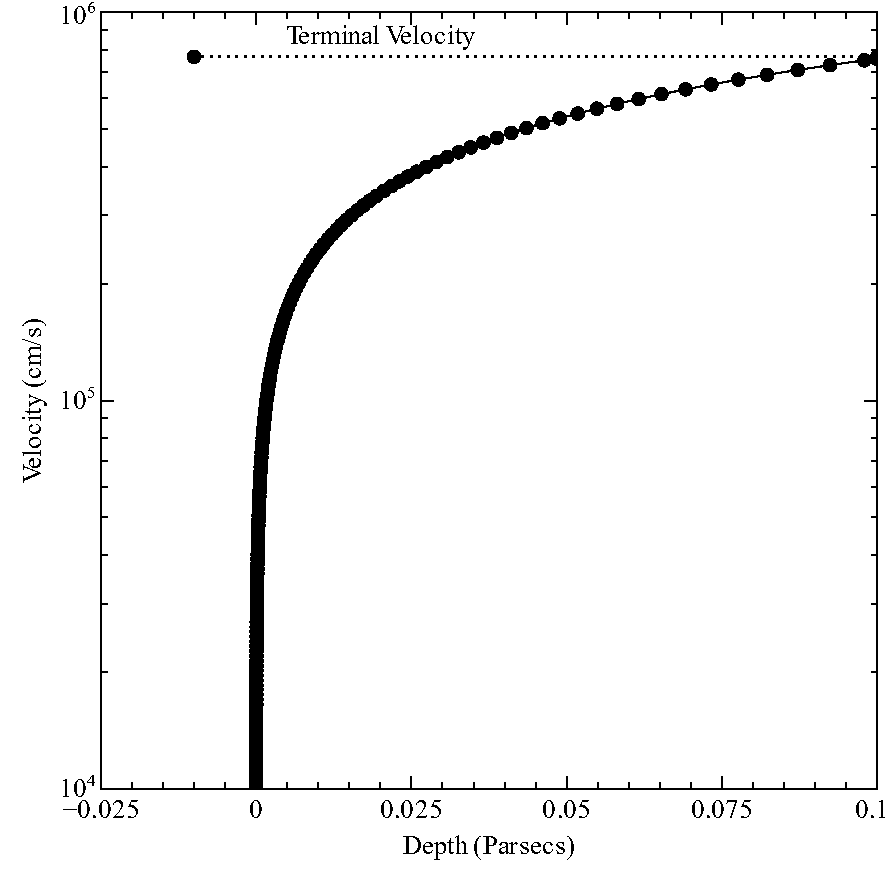
\includegraphics[scale=0.75]{WindVelocityvsDepth}
\caption[Wind velocity vs depth]
{The wind velocity is computed using the input stream shown in
one of the test cases in the last section.  Parameters were chosen to have
a readily computed final velocity.  The velocity at the outer edge of the
slab is within 1 percent of its expected value.}
\label{fig:WindVelocityvsDepth}
\end{figure}

\section{Eddington limit}

The Eddington limit is given by
\begin{equation}
{L_{Edd}} = \frac{{4\pi GcM}}{\kappa } = 1.45 \times
{10^{38}}\frac{M}{{{M_o}}}\frac{{{\kappa _T}}}{\kappa }
\quad [\mathrm{erg~s}^{-1}]
\end{equation}
where $\kappa_T$ is the Thomson opacity and $\kappa$ is the actual gas opacity (generally
several orders of magnitude above Thomson).

\section{Jeans length and mass}

The Jeans length and mass are computed for each zone in the calculation.
The smallest computed Jeans length and mass are saved, and a note is printed
at the end of the calculation if the computed structure is Jeans unstable.

The expression for the Jeans length is
\begin{equation}
{\lambda _J} = {\left( {\frac{{\pi \,k\,T}}{{\mu \,{m_u}G\,\rho }}}
\right)^{1/2}} = 6.257 \times {10^7}{\left( {\frac{T}{{\mu \rho }}}
\right)^{1/2}}
\quad [\mathrm{cm}]
\end{equation}
where $\mu$ is the mean mass per particle of the gas
\begin{equation}
\mu  = \frac{{\sum {{n_i}\,{m_i}} }}{{\sum {{n_i}} }}
\quad [\mathrm{gm}].
\end{equation}

The Jeans mass is then given by
\begin{equation}
{M_J} = \frac{{4\pi }}{3}\;\rho \,{\left( {\frac{{{\lambda _J}}}{2}}
\right)^3}
\quad [\mathrm{gm}]
\end{equation}
where the mass is that of a sphere with radius $\lambda_J /2$.

The minimum Jeans mass is evaluated as the calculation progresses.  The
code will generate a comment if the computed structure is Jeans unstable.

\section{Luminosity Distance}

The luminosity distance DL is given by
\begin{equation}
{D_L} = \left\{ \begin{array}{ccccc}
& \frac{{cz}}{{{H_o}}}\left( {1 + z/2} \right)& {q_o} = 0 \\
& \frac{c}{{{H_o}q_o^2}}\left\{ {{q_o}z + \left( {{q_o} - 1} \right)\left[
{{{\left( {2{q_o}z + 1} \right)}^{1/2}} - 1} \right]} \right\}\quad \,\,
& {q_o} > 0 \\
& \frac{{2c}}{{{H_o}}}\left[ {1 + z - {{\left( {1 + z} \right)}^{1/2}}}
\right]& {q_o} = 1/2 \\
 \end{array} \right.
\quad [\mathrm{cm}]
\end{equation}
For $q_o=1/2$ and $H_o = 70$ km/s/Mpc the luminosity distance is
\begin{equation}
{D_L} = 2.643 \times {10^{26}}\left[ {1 + z - {{\left( {1 + z}
\right)}^{1/2}}} \right]
\quad  [\mathrm{cm}]
\end{equation}
The proper distance $D_P$ is given by ${D_P} = {D_L}\left( {1 + z} \right)$.

\citet{Liske2000} provides expressions giving the cosmological distance and
redshift between any two objects.
\citet{Hogg1999} gives a nice pedagogical
review of distance measures in cosmology.

